\chapter{Particle Physics Solutions}
\begin{abox}
	Practise set-1
\end{abox}
\begin{enumerate}
	\item  Consider the decay $A \rightarrow B+C$ of a relativistic spin $-\frac{1}{2}$ particle $A$. Which of the following statements is true in the rest frame of the particle $A$ ?
	{\exyear{ NET/JRF (JUNE-2019)}}	
	\begin{tasks}(1)
		\task[\textbf{a.}]The spin of both $B$ and $C$ may be $\frac{1}{2}$
		\task[\textbf{b.}]The sum of the masses of $B$ and $C$ is greater than the mass of $A$
		\task[\textbf{c.}]The energy of $B$ is uniquely determined by the masses of the particles
		\task[\textbf{d.}]  The spin of both $B$ and $C$ may be integral
	\end{tasks}
	\begin{answer}
		So the correct answer is \textbf{Option (c)}
	\end{answer}
	\item  The charm quark $S$ assigned a charm quantum number $C=1$. How should the Gellmann-Nishijima formula for electric charge be modified for four flavors of quarks?
	{\exyear{ NET/JRF (JUNE-2015)}}
	\begin{tasks}(2)
		\task[\textbf{a.}]$I_3+\frac{1}{2}(B-S-C)$
		\task[\textbf{b.}]$I_3+\frac{1}{2}(B-S+C)$
		\task[\textbf{c.}] $I_3+\frac{1}{2}(B+S-C)$
		\task[\textbf{d.}]$I_3+\frac{1}{2}(B+S+C)$ 
	\end{tasks}
	\begin{answer}
		\begin{align*}
		\text{From Gell-Mann-Nishijima formula }Q&=I_3+\frac{1}{2}(B+S)\\
		\text{For Quark it is generalized as }Q&=I_3+\frac{1}{2}(B+S+C)
		\end{align*}
		So the correct answer is \textbf{Option (d)}
	\end{answer}
	\item  A spin-1/2 particle $A$ undergoes the delay $A \rightarrow B+C+D$, where it is known that $B$ and $C$ are also spin-1/2 particles. The complete set of allowed values of the spin of the particle $D$ is
	{\exyear{ NET/JRF (JUNE-2013)}}
	\begin{tasks}(2)
		\task[\textbf{a.}]$\frac{1}{2}, 1, \frac{3}{2}, 2, \frac{5}{2}, 3, \ldots$
		\task[\textbf{b.}]0,1
		\task[\textbf{c.}]$\frac{1}{2}$ only
		\task[\textbf{d.}]$\frac{1}{2}, \frac{3}{2}, \frac{5}{2}, \frac{7}{2}, \ldots$ 
	\end{tasks}
	\begin{answer}
		Spin of the left side and combined spin of the products must be same to conserve the spin angular momentum conservation law.\\\\
		So the correct answer is \textbf{Option (c)}
	\end{answer}
	\item  A baryon $X$ decays by strong interaction as $X \rightarrow \Sigma^{+}+\pi^{-}+\pi^0$, where $\Sigma^{+}$is a member of the isotriplet $\left(\Sigma^{+}, \Sigma^0, \Sigma^{-}\right)$. The third component $I_3$ of the isospin of $X$ is
	{\exyear{ NET/JRF (JUNE-2017)}}
	\begin{tasks}(4)
		\task[\textbf{a.}]0
		\task[\textbf{b.}] $1 / 2$
		\task[\textbf{c.}]1
		\task[\textbf{d.}] $3 / 2$
	\end{tasks}
	\begin{answer}
		\begin{align*}
		&X=\sum^{+}+\pi^{-}+\pi^0\\
		&I_3: 1\quad-1 \quad 0\\
		&\Rightarrow I_3 \text { for } X \text { is } 0 \text {. }
		\end{align*}
		So the correct answer is \textbf{Option (a)}
	\end{answer}
	\item  The reaction ${ }_1^2 D+{ }_1^2 D \rightarrow{ }_2^4 \mathrm{He}+\pi^0$ cannot proceed via strong interactions because it violates the conservation of
	{\exyear{ NET/JRF (JUNE-2015)}}
	\begin{tasks}(2)
		\task[\textbf{a.}]Angular momentum
		\task[\textbf{b.}]Electric charge
		\task[\textbf{c.}]Baryon number
		\task[\textbf{d.}] Isospin 
	\end{tasks}
	\begin{answer}
		\begin{align*}
		&{ }_1 D^2+{ }_1 D^2 \rightarrow{ }_2 \mathrm{He}^4+\pi^0
		\text{(Not conserved)}\\
		&I: 0 \quad 0 \rightarrow 0 \quad 1\\
		&\text{This isopin is not conserved in above reaction.}
		\end{align*}
		So the correct answer is \textbf{Option (d)}
	\end{answer}
	\item  A beam of pions $\left(\pi^{+}\right)$is incident on a proton target, giving rise to the process
	$$
	\pi^{+}+p \rightarrow n+\pi^{+}+\pi^{+}
	$$
	Assuming that the decay proceeds through strong interactions, the total isospin $I$ and its third component $I_3$ for the decay products, are
	{\exyear{ NET/JRF (JUNE-2011)}}
	\begin{tasks}(2)
		\task[\textbf{a.}] $I=\frac{3}{2}, I_3=\frac{3}{2}$
		\task[\textbf{b.}]$I=\frac{5}{2}, I_3=\frac{5}{2}$
		\task[\textbf{c.}]$I=\frac{5}{2}, I_3=\frac{3}{2}$
		\task[\textbf{d.}] $I=\frac{1}{2}, I_3=-\frac{1}{2}$
	\end{tasks}
	\begin{answer}
		\begin{align*}
		\pi^{+}+p \rightarrow n+\pi^{+}+\pi^{+} ; \quad I: \frac{1}{2}+1+1=\frac{5}{2}, \quad I_3:-\frac{1}{2}+1+1=\frac{3}{2}
		\end{align*}
		So the correct answer is \textbf{Option (c)}
	\end{answer}
	\item  A beam of pions $\left(\pi^{+}\right)$is incident on a proton target, giving rise to the process
	$$
	\pi^{+}+p \rightarrow n+\pi^{+}+\pi^{+}
	$$
	Using isospin symmetry, the cross-section for the above process can be related to that of the process
	\begin{tasks}(2)
		\task[\textbf{a.}]$\pi^{-} n \rightarrow p \pi^{-} \pi^{-}$
		\task[\textbf{b.}]$\pi^{-} \bar{p} \rightarrow \bar{n} \pi^{-} \pi^{-}$
		\task[\textbf{c.}]$\pi^{+} n \rightarrow p \pi^{+} \pi^{-}$
		\task[\textbf{d.}]  $\pi^{+} \bar{p} \rightarrow n \pi^{+} \pi^{-}$
	\end{tasks}
	\begin{answer}
		So the correct answer is \textbf{Option (c)}
	\end{answer}
	\item  The dominant interactions underlying the following processes
	A. $K^{-}+p \rightarrow \sum^{-}+\pi^{+}$, B. $\mu^{-}+\mu^{+} \rightarrow K^{-}+K^{+}$, C. $\Sigma^{+} \rightarrow p+\pi^0$ are
	{\exyear{ NET/JRF (JUNE-2012)}}
	\begin{tasks}(1)
		\task[\textbf{a.}]A: strong, B: electromagnetic and; C: weak
		\task[\textbf{b.}]A: strong, B: weak and; C: weak
		\task[\textbf{c.}]A: weak, B: electromagnetic and; C: strong
		\task[\textbf{d.}]  A: weak, B: electromagnetic and; C: weak
	\end{tasks}
	\begin{answer}
		\begin{align*}
		&\text{(A)\quad }K^{-}+p \rightarrow \sum^{-}+\pi^{+} \quad\text{ (Strong interaction)}\\
		&\quad I_3:-\frac{1}{2}+\frac{1}{2} \rightarrow-1+1 \text { (Conserved) }\\
		&\text{(B)\quad }\mu^{-}+\mu^{+} \rightarrow K^{-}+K^{+}
		\text{	(Electromagnetic interaction)}\\
		&\text{(C)\quad }\Sigma^{+} \rightarrow p+\pi^0
		\text{	(Weak interaction)}\\
		&\quad I_3: 1 \rightarrow \frac{1}{2}+0
		\text{(Not conserved)}
		\end{align*}
		So the correct answer is \textbf{Option (a)}
	\end{answer}
	\item  Consider the four processes\\
	(i) $p^{+} \rightarrow n+e^{+}+v_e$\\
	(ii) $\Lambda^0 \rightarrow p^{+}+e^{+}+v_e$\\
	(iii) $\pi^{+} \rightarrow e^{+}+v_e$\\
	(iv) $\pi^0 \rightarrow \gamma+\gamma$\\
	which of the above is/are forbidden for free particles?
	{\exyear{NET/JRF (DEC-2014)}}
	\begin{tasks}(2)
		\task[\textbf{a.}]Only (ii)
		\task[\textbf{b.}](ii) and (iv)
		\task[\textbf{c.}](i) and (iv)
		\task[\textbf{d.}]  (i) and (ii)
	\end{tasks}
	\begin{answer}
		\begin{align*}
		&\text{(i) $p^{+} \rightarrow n+e^{+}+v_e$ [Not allowed]}
		\intertext{It violate energy conservation. The mass of proton is less than mass of neutron. Free proton is stable and can not decay to neutron. Proton can decay to neutron only inside the nucleus, where energy violation is taken care by Heisenberg uncertainty principle.}
		&\text{(ii) $\Lambda^0 \rightarrow p^{+}+e^{+}+v_e$ [Not allowed]. In this decay charge is not conserved}\\
		&\text{(iii) $\pi^{+} \rightarrow e^{+}+v_e$ [allowed through Weak interaction]}\\
		&\text{(iv) $\pi^0 \rightarrow \gamma+\gamma$ [allowed through Electromagnetic interaction]}
		\end{align*}
		So the correct answer is \textbf{Option (d)}
	\end{answer}
	\item  Consider the following processes involving free particles\\
	(i) $\bar{n} \rightarrow \bar{p}+e^{+}+\bar{v}_e$\\
	(ii) $\bar{p}+n \rightarrow \pi^{-}$\\
	(iii) $p+n \rightarrow \pi^{+}+\pi^0+\pi^0$\\
	(iv) $p+\bar{v}_e \rightarrow n+e^{+}$\\
	Which of the following statements is true?
	{\exyear{ NET/JRF (DEC-2015)}}
	\begin{tasks}(1)
		\task[\textbf{a.}] Process (i) obeys all conservation laws
		\task[\textbf{b.}]Process (ii) conserves baryon number, but violates energy-momentum conservation
		\task[\textbf{c.}] process (iii) is not allowed by strong interaction but is allowed by weak interactions
		\task[\textbf{d.}] Process (iv) conserves baryon number, but violates lepton number conservation
	\end{tasks}
	\begin{answer}
		\begin{align*}
		&\text { (i)}\quad  \bar{n} \rightarrow \bar{p}+e^{+}+\bar{v}_e\\
		&\begin{array}{lllll}
		q & 0 &-1&+1&
		0 \text{ (conserved)}\\
		\text { spin }&-\frac{1}{2}&-\frac{1}{2}&-\frac{1}{2}&-\frac{1}{2} \text { (not conserved) }\\
		\text { Le } &0 &0 &-1 & -1 \text { (not conserved) }
		\end{array}\\
		&\text{(ii) Baryon number is conserved but energy and momentum conservation violated.}\\
		&\text{(iii) spin is not conserved}\\
		&\text{(iv) obeys all conservation laws.}
		\end{align*}
		So the correct answer is \textbf{Option (b)}
	\end{answer}
	\item Which of the following reaction(s) is/are allowed by the conservation laws?
	(i) $\pi^{+}+n \rightarrow \Lambda^0+K^{+}$
	(ii) $\pi^{-}+p \rightarrow \Lambda^0+K^0$
	{\exyear{ NET/JRF (DEC-2016)}}
	\begin{tasks}(2)
		\task[\textbf{a.}]Both (i) and (ii)
		\task[\textbf{b.}] Only (i)
		\task[\textbf{c.}] Only (ii)
		\task[\textbf{d.}]  Neither (i) nor (ii)
	\end{tasks}
	\begin{answer}
		\begin{align*}
		&\text{(i)}\pi^{+}+n \rightarrow \Lambda^0+K^{+}\\
		&q: 1+0 \rightarrow 0+1 \\
		&B: 0+1 \rightarrow 1+0 \\
		&S: 0+0 \rightarrow-1+1\\
		&\text{Reaction is allowed}\\
		&\text{(ii)} \pi^{-}+p \rightarrow \Lambda^0+K^0\\
		&q:-1+1 \rightarrow 0+0\\
		&B: 0+1 \rightarrow 1+0\\
		&S: 0+0 \rightarrow-1+1\\
		&\text{Reaction is allowed}
		\end{align*}
		So the correct answer is \textbf{Option (a)}
	\end{answer}
	\item  Which of the following process is not allowed by the strong interaction but is allowed by the weak interaction?
	{\exyear{ NET/JRF (DEC-2017)}}
	\begin{tasks}(2)
		\task[\textbf{a.}]$K^0+\pi^0 \rightarrow \bar{K}^0+\pi^{+}+\pi^{-}$
		\task[\textbf{b.}]$p+n \rightarrow d+p+\bar{p}$
		\task[\textbf{c.}]$\Delta^{+}+K^0 \rightarrow p+n$
		\task[\textbf{d.}] $p+\Delta^{+} \rightarrow \bar{n}+\Delta^{++}$
	\end{tasks}
	\begin{answer}
		\begin{align*}
		&\text { (1) } K^0+\pi^0 \rightarrow \bar{K}^0+\pi^{+}+\pi^{-}\\
		&\begin{array}{lllllll}
		\text { Charge }& 0 & 0 & 0 & +1 & -1 & \text { Conserved }\\
		\text { Spin }0 & 0 & 0 & 0 & 0 &0& \text { Conserved }\\
		I & \frac{1}{2} & 1 & \frac{1}{2} & 1 & 1&\text { Not conserved }\\
		I_3 & \frac{-1}{2} & 0 & +\frac{1}{2} & +1 & -1 & \Delta I_3=1 \\
		S & +1 & 0 & -1 & 0 & 0 & \Delta S=1
		\end{array}\\
		&\text{This interaction is not allowed by strong interaction but allowed by weak interaction}
		\end{align*}
		So the correct answer is \textbf{Option (a)}
	\end{answer}
	\item  Which of the following elementary particle processes does not conserve strangeness?
	{\exyear{ NET/JRF (JUNE-2018)}}
	\begin{tasks}(2)
		\task[\textbf{a.}]$\pi^0+p \rightarrow k^{+}+\wedge^0$
		\task[\textbf{b.}]$\pi^{-}+p \rightarrow k^0+\wedge^0$
		\task[\textbf{c.}]$\Delta^0 \rightarrow \pi^0+n$
		\task[\textbf{d.}] $K^0 \rightarrow \pi^{+}+\pi^{-}$
	\end{tasks}
	\begin{answer}
		\begin{align*}
		&\text{(a)}\\
		&\begin{array}{rrrrrrr} 
		&\pi^0&+p & \rightarrow & k^{+}&+\wedge^0&   \\
		S:&0&0& &+1&-1&\text{Conserved}\\
		\end{array}\\
		&\text{(b)}\\
		&\begin{array}{rrrrrrr} 
		&\pi^-&+p & \rightarrow & k^{0}&+\wedge^0&   \\
		S:&0&0& &+1&-1&\text{Conserved}\\
		\end{array}\\
		&\text{(c)}\\
		&\begin{array}{rrrrrrr} 
		&\Delta ^0& \rightarrow & \pi^{0}&+n&   \\
		S:&0& &0&0&\text{Conserved}\\
		\end{array}\\
		&\text{(d)}\\
		&\begin{array}{rrrrrrr} 
		&K ^0& \rightarrow & \pi^{+}&+\pi^-&   \\
		S:&+1& &0&0&\text{Not Conserved}\\
		\end{array}\\
		\end{align*}
		So the correct answer is \textbf{Option (d)}
	\end{answer}
	\item  Which of the following decay processes is allowed?
	\begin{tasks}(2)
		\task[\textbf{a.}]$K^0 \rightarrow \mu^{+}+\mu^{-}$
		\task[\textbf{b.}] $\mu^{-} \rightarrow e^{-}+\gamma$
		\task[\textbf{c.}]$n \rightarrow p+\pi^{-}$
		\task[\textbf{d.}] $n \rightarrow \pi^{+}+\pi^{-}$
	\end{tasks}
	\begin{answer}
		\begin{align*}
		&\begin{array}{lllll}
		q:&0&+1&-1&\text{:Conserved}\\
		\text{Spin:}&0&\frac{1}{2}&\frac{1}{2}&\text{:Conserved}\\
		L_\mu:&0&-1&+1&\text{:Conserved}\\
		I:&\frac{1}{2}&0&0&:\text{Not Conserved}\\
		I_3:&\frac{-1}{2}&0&0&:\text{Not Conserved}\\
		S:&+1&0&0&:\text{Not Conserved}\\
		\end{array}\\
		&\text { Thus this is an allowed decay through weak interaction. }
		\end{align*}
		So the correct answer is \textbf{Option (a)}
	\end{answer}
	\item  The recently-discovered Higgs boson at the LHC experiment has a decay mode into a photon and a $Z$ boson. If the rest masses of the Higgs and $Z$ boson are $125 \mathrm{GeV} / \mathrm{c}^2$ and $90 \mathrm{GeV} / \mathrm{c}^2$ respectively, and the decaying Higgs particle is at rest, the energy of the photon will approximately be
	{\exyear{ NET/JRF (JUNE-2014)}}
	\begin{tasks}(2)
		\task[\textbf{a.}] $35 \sqrt{3} \mathrm{GeV}$
		\task[\textbf{b.}]$35 \mathrm{GeV}$
		\task[\textbf{c.}] $30 \mathrm{GeV}$
		\task[\textbf{d.}] $15 \mathrm{GeV}$
	\end{tasks}
	\begin{answer}
		\begin{align*}
		\text { Assume } \mathrm{H} &\text { is symbol of Higgs boson, } H \rightarrow Z+\gamma\\
		E_\gamma&=\frac{E_H^2-E_Z^2}{2 E_H}=\frac{(125)^2-(90)^2}{2 \times 125}=30 \mathrm{GeV}
		\end{align*}
		So the correct answer is \textbf{Option (c)}
	\end{answer}
	\item  In the large hadron collider $(L H C)$, two equal energy proton beams traverse in opposite directions along a circular path of length $27 \mathrm{~km}$. If the total centre of mass energy of a proton-proton pair is $14 \mathrm{TeV}$, which of the following is the best approximation for the proper time taken by a proton to traverse the entire path?
	{\exyear{ NET/JRF (JUNE-2016)}}
	\begin{tasks}(4)
		\task[\textbf{a.}]$12 n s$
		\task[\textbf{b.}]$1.2 \mu \mathrm{s}$
		\task[\textbf{c.}]$1.2 \mathrm{~ns}$
		\task[\textbf{d.}] $0.12 \mu \mathrm{s}$ 
	\end{tasks}
	\begin{answer}
		\begin{align*}
		\text{The proton travel at nearly speed  }&\text{of light in $L H C$, therefore}\\
		t \approx \frac{d}{c}&=\frac{27 \times 10^3}{3 \times 10^8} \approx 9 \times 10^{-5} \mathrm{sec}\\
		\text{Since, proton is relativistic, }t_0&=t \sqrt{1-\frac{v^2}{c^2}}=\frac{t}{\gamma}\\
		\because \quad E=\gamma m_0 c^2 \Rightarrow \frac{1}{\gamma}&=\frac{m_0 c^2}{E}=\frac{938 \mathrm{MeV}}{7 \mathrm{TeV}}=\frac{938 \times 10^6 \mathrm{eV}}{7 \times 10^{12} \mathrm{eV}}=1.34 \times 10^{-4}\\
		\text{Thus, }t_0=\frac{t}{\gamma}&=9 \times 10^{-5} \times 1.34 \times 10^{-4}=1.2 \times 10^{-8} \mathrm{sec}=12 \mathrm{~ns}
		\end{align*}
		So the correct answer is \textbf{Option (a)}
	\end{answer}
	\item  Muons are produced through the annihilation of particle $a$ and its anti-particle, namely the process $a+\bar{a} \rightarrow \mu^{+}+\mu^{-}$. A muon has a rest mass of $105 \mathrm{MeV} / \mathrm{c}^2$ and its proper life time is $2 \mu \mathrm{s}$. If the center of mass energy of the collision is $2.1 \mathrm{GeV}$ in the laboratory frame that coincides with the center-of-mass frame, then the fraction of muons that will decay before they reach a detector placed $6 \mathrm{~km}$ away from the interaction point is
	{\exyear{ NET/JRF (JUNE-2013)}}
	\begin{tasks}(4)
		\task[\textbf{a.}]$e^{-1}$
		\task[\textbf{b.}]$1-e^{-1}$
		\task[\textbf{c.}] $1-e^{-2}$
		\task[\textbf{d.}]  $e^{-10}$
	\end{tasks}
	\begin{answer}
		\begin{align*}
		N&=N_0 e^{-\lambda t} \Rightarrow \frac{N}{N_0}=e^{-\lambda t}=e^{-\frac{t}{\gamma t}} \text {, where } \tau=2 \times 10^{-6} s, \gamma=\frac{2.1}{105} \times 10^3=20 \text { and }\\
		t&=\frac{6 \times 10^3}{3 \times 10^8}=2 \times 10^{-5} \mathrm{sec} \text {. Thus } \frac{t}{\gamma \tau}=\frac{1}{2} \Rightarrow \frac{N}{N_0}=e^{-\frac{1}{2}} \approx 1-e^{-1}
		\end{align*}
		So the correct answer is \textbf{Option (b)}
	\end{answer}
	\item  In a classical model, a scalar (spin-0) meson consists of a quark and an antiquark bound by a potential $V(r)=a r+\frac{b}{r}$, where $a=200 \mathrm{MeV} \mathrm{fm}^{-1}$ and $b=100 \mathrm{MeV} \mathrm{fm}$. If the masses of the quark and antiquark are negligible, the mass of the meson can be estimated as approximately
	{\exyear{ NET/JRF (JUNE-2014)}}
	\begin{tasks}(4)
		\task[\textbf{a.}]$141 \mathrm{MeV} / \mathrm{c}^2$
		\task[\textbf{b.}] $283 \mathrm{MeV} / \mathrm{c}^2$
		\task[\textbf{c.}]$353 \mathrm{MeV} / \mathrm{c}^2$
		\task[\textbf{d.}] $425 \mathrm{MeV} / \mathrm{c}^2$
	\end{tasks}
	\begin{answer}
		At equilibrium separation the potential is minimum, thus the equilibrium separation can be determined as
		\begin{align*}
		\left.\frac{d V(r)}{d r}\right|_{r=r_0}=a-\frac{b}{r_0^2}=0 \Rightarrow r_0&=\sqrt{\frac{b}{a}}=\sqrt{\frac{100 \mathrm{MeVfm}}{200 \mathrm{MeVfm}^{-1}}}=\frac{1}{\sqrt{2}} \mathrm{fm}\\
		\text{The equilibrium separation between}&\text{ particles is also estimated by uncertainty principle}\\
		r_0=c \Delta t \quad \Rightarrow \quad r_0&=c \frac{\hbar}{\Delta E} \quad(\text { where, } \Delta E \Delta t \approx \hbar)\\
		\text{Where, $\mathrm{c}$ is the velocity of the virtual meson}\\
		r_0=c \frac{\hbar}{\Delta E}&=\frac{200 \mathrm{MeV} \cdot f m}{\Delta E(\mathrm{MeV})}\\
		\text{Using above two relation }\frac{200 \mathrm{MeV} \cdot f m}{\Delta E(\mathrm{MeV})}&=\frac{1}{\sqrt{2}} f m\\
		\Delta E=200 \sqrt{2}&=283 \mathrm{MeV} \Rightarrow \Delta E=\Delta m \times c^2\\
		\text{the mass of the meson }\Delta m&=\frac{\Delta E}{c^2}=283 \mathrm{MeV} / \mathrm{c}^2
		\end{align*}
		So the correct answer is \textbf{Option (b)}
	\end{answer}
	\item  The range of the nuclear force between two nucleons due to the exchange of pions is $1.40 \mathrm{fm}$. If the mass of pion is $140 \mathrm{MeV} / \mathrm{c}^2$ and the mass of the rho-meson is $770 \mathrm{MeV} / \mathrm{c}^2$, then the range of the force due to exchange of rho-mesons is
	{\exyear{ NET/JRF (JUNE-2017)}}
	\begin{tasks}(4)
		\task[\textbf{a.}]$1.40 \mathrm{fm}$
		\task[\textbf{b.}]$7.70 \mathrm{fm}$
		\task[\textbf{c.}]$0.25 \mathrm{fm}$
		\task[\textbf{d.}]$0.18 \mathrm{fm}$ 
	\end{tasks}
	\begin{answer}
		\begin{align*}
		\text{Range for nuclear force between nucleon will be }R&=c \Delta t=\frac{\hbar c}{m c^2}\text{ and }\hbar c=199 \mathrm{MeVfm}\\
		\Rightarrow R&=\frac{199 \mathrm{MeVfm}}{770 \frac{\mathrm{MeV}}{c^2} \times c^2} \approx 0.25 \mathrm{fm}
		\end{align*}
		So the correct answer is \textbf{Option (c)}
	\end{answer}
	\item  The mean life-time of the following decays: $\rho_0 \rightarrow \pi^{+}+\pi^{-}, \pi^0 \rightarrow \gamma+\gamma, \mu^{-} \rightarrow e^{-}+\bar{v}_e+v_\mu$, are $\tau_\rho, \tau_\pi$ and $\tau_\mu$ respectively.
	They satisfy
	{\exyear{ NET/JRF (JUNE-2019)}}
	\begin{tasks}(2)
		\task[\textbf{a.}]$\tau_\pi<\tau_\rho<\tau_\mu$
		\task[\textbf{b.}]$\tau_\mu<\tau_\rho<\tau_\pi$
		\task[\textbf{c.}]$\tau_\rho<\tau_\pi<\tau_\mu$
		\task[\textbf{d.}] $\tau_\rho<\tau_\mu<\tau_\pi$
	\end{tasks}
	\begin{answer}
		\begin{align*}
		&\text{The characteristic time for strong, electromagnetic and weak interaction are} \\
		&\text{$\approx 10^{-23} \mathrm{sec}, 10^{-20} \mathrm{sec}$ and $10^{-11} \mathrm{sec}$}\\
		&\text{$\rho_0 \rightarrow \pi^{+}+\pi^{-}$is strong interaction with $\tau_\rho \simeq 10^{-23} \mathrm{sec}$}\\
		&\text{$\pi^0 \rightarrow \gamma+\gamma$ is electromagnetic interaction with $\tau_\pi \simeq 10^{-20} \mathrm{sec}$}\\
		&\text{$\mu^{-} \rightarrow e^{-}+\bar{v}_e+v_\mu$ is weak interaction with $\tau_\mu \simeq 10^{-11} \mathrm{sec}$}\\
		&\text{Thus, $\tau_\rho<\tau_\pi<\tau_\mu$. The correct option is (c)}
		\end{align*}
		So the correct answer is \textbf{Option (c)}
	\end{answer}
	\item  A particle, which is a composite state of three quarks $u, d$ and $s$, has electric charge, spin and strangeness respectively, equal to
	{\exyear{ NET/JRF (DEC-2016)}}
	\begin{tasks}(2)
		\task[\textbf{a.}]$1, \frac{1}{2},-1$
		\task[\textbf{b.}]$0,0,-1$
		\task[\textbf{c.}]$0, \frac{1}{2},-1$
		\task[\textbf{d.}] $-1,-\frac{1}{2}+1$
	\end{tasks}
	\begin{answer}
		Charge, spin and strangers of Quarks $u,d$ and $s$ are given as
		\begin{align*}
		&\begin{array}{ccccc} 
		& \mathrm{U} & \mathrm{D} & \mathrm{S} & \text { Total } \\
		\text { Charge } & \frac{+2}{3} & \frac{-1}{3} & \frac{-1}{3} & 0\\
		\text { Spin } & \frac{1}{2} & \frac{1}{2} & \frac{1}{2} & \frac{1}{2} \text { or } \frac{3}{2} \\
		\text { Strangeness } & 0 & 0 & -1 & -1
		\end{array}\\
		&\text{If a particle $x$ is a composite of $u, d \& s$, then net charge, spin and strangeness on $x$ is net charge $=0$}\\
		&\text{net spin $=\frac{1}{2}$ or $\frac{3}{2}$ and net strangeness $=-1$}
		\end{align*}
		So the correct answer is \textbf{Option (c)}
	\end{answer}
	\item  The elastic scattering of a neutrino $v_e$ by an electron $e^{-}$, i.e. the reaction $v_e+e^{-} \rightarrow v_e+e^{-}$can be described by the interaction Hamiltonian
	$$
	H_{\mathrm{int}}=\frac{1}{\sqrt{2}} G_F \int d^3 x\left(\bar{\psi}_e(x) \gamma^\mu \psi_{v e}(x)\right)\left(\bar{\psi}_{v e}(x) \gamma_\mu \psi_e(x)\right)
	$$
	The cross-section of the above process depends on the centre of mass energy $E$, as
	{\exyear{ NET/JRF (JUNE-2019)}}
	\begin{tasks}(4)
		\task[\textbf{a.}]$\frac{1}{E^2}$
		\task[\textbf{b.}]$E^2$
		\task[\textbf{c.}]$E$
		\task[\textbf{d.}] $\sqrt{E}$
	\end{tasks}
	\begin{answer}
		Feynman diagram for the process of electron-neutron scattering.\\
		\begin{figure}[H]
			\centering
			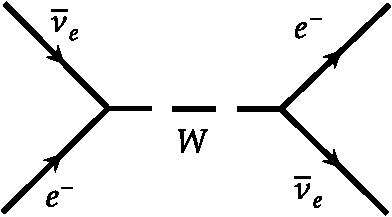
\includegraphics[height=2.5cm,width=4cm]{diagram-20221031-2-crop}
		\end{figure}
		The kinematics of elastic neutrino electron scattering is fully described by a single variable; for instance, by $\theta_e$, the angle of the outgoing electron with respect to the neutrino beam. If $E_v$ and $E_e$ be the energies of the incoming neutrino and outgoing electron, $m_e$ the electron mass, and $y=E_e / E_v$ be the fractional energy loss of the neutrino in the laboratory frame. From the effective Lagrangian the differential crosssection, often called y-distribution for the case of high neutrino energy $\left(E_v \gg E_e\right)$
		\begin{align*}
		\frac{d \sigma}{d y}=g_{L, R}^2 \frac{2 G_F^2 m_e}{\pi} E_v \quad \Rightarrow \sigma \propto E_v
		\end{align*}
		So the correct answer is \textbf{Option (c)}
	\end{answer}
	\item  A deuteron $d$ captures a charged pion $\pi^{-}$in the $l=1$ state, and subsequently decays into a pair of neutrons $(n)$ via strong interaction. Given that the intrinsic parities of $\pi^{-}, d$ and $n$ are $-1,+1$ and $+1$ respectively, the spin wavefunction of the final state neutrons is
	{\exyear{ NET/JRF (JUNE-2018)}}
	\begin{tasks}(2)
		\task[\textbf{a.}]Linear combination of a singlet and a triplet
		\task[\textbf{b.}]Singlet
		\task[\textbf{c.}]Triplet
		\task[\textbf{d.}] Doublet
	\end{tasks}
	\begin{answer}
		\begin{align*}
		\text{ Parity must conserve intersections}\\
		\pi+d &\rightarrow n+n\\
		\text{	The parity of the initial state is}\\
		(-1)^l P_\pi P_d&=(-1)^1(-1)(+1)=+1\\
		\text{The parity of the final state is}\\
		(-1)^l P_n P_n=(-1)^l(+1)(+1)&=(-1)^l=1 \hspace{2cm} \because l=0,2, \ldots .
		\intertext{because the nucleons are identical fermions, the allowed states of two nucleons are ${ }^1 S_0,{ }^3 P_{0,1,2}$ corresponding to $l=0$ and $l=1$. Thus only $l=0$ (singlet) is allowed.}
		\end{align*}
		So the correct answer is \textbf{Option (b)}
	\end{answer}
	\item  Charged pions $\pi^{-}$decay to muons $\mu^{-}$and anti-muon neutrinos $\vec{v}_\mu ; \pi^{-} \rightarrow \mu^{-}+\vec{v}_\mu$. Take the rest masses of a muon and a pion to be $105 \mathrm{MeV}$ and $140 \mathrm{MeV}$, respectively. The probability that the measurement of the muon spin along the direction of its momentum is positive, is closest to
	NET/JRF (JUNE-2020)
	\begin{tasks}(4)
		\task[\textbf{a.}]$0.5$
		\task[\textbf{b.}]$0.75$
		\task[\textbf{c.}]1
		\task[\textbf{d.}] 0
	\end{tasks}
	\begin{answer}
		So the correct answer is \textbf{Option (c)}
	\end{answer}
	\colorlet{ocre1}{ocre!70!}
	\colorlet{ocrel}{ocre!30!}
	\setlength\arrayrulewidth{1pt}
	\begin{table}[H]
		\centering
		\arrayrulecolor{ocre}
		\begin{tabular}{|p{1.5cm}|p{1.5cm}||p{1.5cm}|p{1.5cm}|}
			\hline
			\multicolumn{4}{|c|}{\textbf{Answer key}}\\\hline\hline
			\rowcolor{ocrel}Q.No.&Answer&Q.No.&Answer\\\hline
			1&\textbf{c} &2&\textbf{d}\\\hline 
			3&\textbf{c} &4&\textbf{a} \\\hline
			5&\textbf{d} &6&\textbf{c} \\\hline
			7&\textbf{c}&8&\textbf{a}\\\hline
			9&\textbf{d}&10&\textbf{b}\\\hline
			11&\textbf{a} &12&\textbf{a}\\\hline
			13&\textbf{d}&14&\textbf{a}\\\hline
			15&\textbf{c}&16&\textbf{a}\\\hline
			17&\textbf{b}&18&\textbf{b}\\\hline
			19&\textbf{c}&20&\textbf{c}\\\hline
			21&\textbf{c} &22&\textbf{c}\\\hline
			23&\textbf{b}&24&\textbf{c}\\\hline
		\end{tabular}
	\end{table}
	
	
	
	
	
	
	
	
	
	
	
	
	
	
	
	
	
\end{enumerate}












































































\begin{abox}
	Practise set-2
\end{abox}
\begin{enumerate}
	\item  Which one of the following sets corresponds to fundamental particles?
	{\exyear{ 	GATE-2012}}
	\begin{tasks}(2)
		\task[\textbf{a.}]Proton, electron and neutron
		\task[\textbf{b.}]Proton, electron and photon
		\task[\textbf{c.}]Electron, photon and neutrino
		\task[\textbf{d.}]Quark, electron and meson 
	\end{tasks}
	\begin{answer}
		So the correct answer is \textbf{Option (a)}
	\end{answer}
	\item  Choose the CORRECT statement from the following
	\begin{tasks}(1)
		\task[\textbf{a.}]Neutron interacts through electromagnetic interaction
		\task[\textbf{b.}]Electron does not interact through weak interaction
		\task[\textbf{c.}]Neutrino interacts through weak and electromagnetic interaction
		\task[\textbf{d.}] Quark interacts through strong interaction but not through weak interaction
	\end{tasks}
	\begin{answer}
		So the correct answer is \textbf{Option (d)}
	\end{answer}
	\item  The isospin and the strangeness of $\Omega^{-}$baryon are
	{\exyear{ GATE-2011}}
	\begin{tasks}(4)
		\task[\textbf{a.}]$1,-3$
		\task[\textbf{b.}]$0,-3$
		\task[\textbf{c.}]1,3
		\task[\textbf{d.}]0,3 
	\end{tasks}
	\begin{answer}
		So the correct answer is \textbf{Option (b)}
	\end{answer}
	\item The isospin $(I)$ and baryon number $(B)$ of the up quark is
	{\exyear{ 	GATE-2013}}
	\begin{tasks}(2)
		\task[\textbf{a.}]$I=1, B=1$
		\task[\textbf{b.}]$I=1, B=1 / 3$
		\task[\textbf{c.}]$I=1 / 2, B=1$
		\task[\textbf{d.}]$I=1 / 2, B=1 / 3$ 
	\end{tasks}
	\begin{answer}
		So the correct answer is \textbf{Option (d)}
	\end{answer}
	\item  Which one of the following is a fermions'?
	{\exyear{ 	GATE-2014}}
	\begin{tasks}(2)
		\task[\textbf{a.}]$\alpha$-particle
		\task[\textbf{b.}]${ }_4 B e^7$ nucleus
		\task[\textbf{c.}]Hydrogen atom
		\task[\textbf{d.}]Deuteron 
	\end{tasks}
	\begin{answer}
		If a nucleus contains odd number of nucleons, it is fermions. If a nucleus contains even number of nucleons, it is a boson.\\
		So the correct answer is \textbf{Option (b)}
	\end{answer}
	\item  In the decay, $\mu^{+} \rightarrow e^{+}+v_e+X$, what is $X$ ?
	{\exyear{ GATE-2018}}
	\begin{tasks}(4)
		\task[\textbf{a.}]$\gamma$
		\task[\textbf{b.}]$\bar{v}_e$
		\task[\textbf{c.}]$v_\mu$
		\task[\textbf{d.}]$\bar{v}_\mu$ 
	\end{tasks}
	\begin{answer}
		\begin{align*}
		u^{+} \rightarrow e^{+}+v_e+\bar{v}_u\\
		\begin{array}{rrrrr}
		L_u: & -1 & 0 & 0 & -1 \\
		L_e: & 0 & -1 & +1 & 0
		\end{array}
		\end{align*}
		So the correct answer is \textbf{Option (d)}
	\end{answer}
	\item  The basic process underlying the neutron $\beta$-decay is
	{\exyear{ GATE-2010}}
	\begin{tasks}(2)
		\task[\textbf{a.}]$d \rightarrow u+e^{-}+\bar{v}_e$
		\task[\textbf{b.}]$d \rightarrow u+e^{-}$
		\task[\textbf{c.}]$s \rightarrow u+e^{-}+\bar{v}_e$
		\task[\textbf{d.}]$u \rightarrow d+e^{-}+\bar{v}_e$ 
	\end{tasks}
	\begin{answer}
		So the correct answer is \textbf{Option (a)}
	\end{answer}
	\item  Match the reactions on the left with the associated interactions on the right.\\
	(1) $\pi^{+} \rightarrow \mu^{+}+v_\mu$\hspace{3cm}
	(i) Strong\\
	(2) $\pi^0 \rightarrow \gamma+\gamma$\hspace{3.5cm}
	(ii) Electromagnetic\\
	(3) $\pi^0+\mathrm{n} \rightarrow \pi^{-}+\mathrm{p}$\hspace{2.6cm}
	(iii) Weak
	{\exyear{ GATE-2010}}
	\begin{tasks}(2)
		\task[\textbf{a.}]$(1$, iii), (2, ii), (3, i)
		\task[\textbf{b.}]$(1$, i), (2, ii), (3, iii)
		\task[\textbf{c.}](1, ii), (2, i), (3, iii)
		\task[\textbf{d.}](1, iii), (2, i), (3, ii) 
	\end{tasks}
	\begin{answer}
		So the correct answer is \textbf{Option (a)}
	\end{answer}
	\item  The quark content of $\Sigma^{+}, K^{-}, \pi^{-}$and $p$ is indicated:
	$$
	\left|\Sigma^{+}\right\rangle=|u u s\rangle ;\left|K^{-}\right\rangle=|s \bar{u}\rangle ;\left|\pi^{-}\right\rangle=|\bar{u} d\rangle ;|p\rangle=|u u d\rangle .
	$$
	In the process, $\pi^{-}+p \rightarrow K^{-}+\Sigma^{+}$, considering strong interactions only, which of the following statements is true?
	{\exyear{ GATE-2012}}
	\begin{tasks}(1)
		\task[\textbf{a.}]The process, is allowed because $\Delta \mathrm{S}=0$
		\task[\textbf{b.}] The process is allowed because $\Delta \mathrm{I}_3=0$
		\task[\textbf{c.}] The process is not allowed because $\Delta \mathrm{S} \neq 0$ and $\Delta \mathrm{I}_3 \neq 0$
		\task[\textbf{d.}]The process is not allowed because the baryon number is violated 
	\end{tasks}
	\begin{answer}
		\begin{align*}
		&\pi^{-}+p \rightarrow k^{-}+\sum^{+}\\
		&\begin{array}{ccccc}
		S: & 0 & 0 & -1 & -1 \text { (not conserved) } \\
		I_3: & -1 & +\frac{1}{2} & -\frac{1}{2} & +1 \text { (not conserved) }
		\end{array}\\
		&\text{For strong interaction $S$ and $I_3$ must conserve. Therefore this process is not allowed }\\
		&\text{under strong interaction}
		\end{align*}
		So the correct answer is \textbf{Option (c)}
	\end{answer}
	\item  The decay process $n \rightarrow p^{+}+e^{-}+\bar{v}_e$ violates
	{\exyear{ 	GATE-2013}}
	\begin{tasks}(2)
		\task[\textbf{a.}]Baryon number
		\task[\textbf{b.}] lepton number
		\task[\textbf{c.}] Isospin
		\task[\textbf{d.}] Strangeness
	\end{tasks}
	\begin{answer}
		So the correct answer is \textbf{Option (c)}
	\end{answer}
	\item  Which one of the following three-quark states $(q q q)$ denoted by $X$ CANNOT be a possible baryon? The corresponding electric charge is indicated in the superscript.
	{\exyear{ 	GATE-2014}}
	\begin{tasks}(4)
		\task[\textbf{a.}]$X^{++}$
		\task[\textbf{b.}]$\mathrm{X}^{+}$
		\task[\textbf{c.}]$X^{-}$
		\task[\textbf{d.}] $\mathrm{X}^{--}$ 
	\end{tasks}
	\begin{answer}
		\begin{align*}
		X^{++}(u u u) \frac{2}{3}+\frac{2}{3}+\frac{2}{3}&=\frac{6}{3}=2(\text{ two unit positive charge })\\
		X^{+}(u u d) \frac{2}{3}+\frac{2}{3}-\frac{1}{3}&=\frac{4}{3}-\frac{1}{3}=1( \text{single unit positive charge })\\
		X^{-}(d d d)&=-\frac{1}{3}-\frac{1}{3}-\frac{1}{3}=-1 (\text{single unit negative charge })\\
		X^{--}\text{[Not possible with }&\left.q q q\right]. 
		\end{align*}
		So the correct answer is \textbf{Option (d)}
	\end{answer}
	\item  The decay $\mu^{+} \rightarrow e^{+}+\gamma$ is forbidden, because it violates
	{\exyear{ 	GATE-2015}}
	\begin{tasks}(1)
		\task[\textbf{a.}] Momentum and lepton number conservations
		\task[\textbf{b.}]Baryon and lepton number conservations
		\task[\textbf{c.}]Angular momentum conservation
		\task[\textbf{d.}]  Lepton number conservation
	\end{tasks}
	\begin{answer}
		\begin{align*}
		\mu^{+} \rightarrow e^{+}+\gamma \text {. In this decay lepton number is not conserved. }
		\end{align*}
		So the correct answer is \textbf{Option (d)}
	\end{answer}
	\item  In the $S U(3)$ quark model, the triplet of mesons $\left(\pi^{+}, \pi^0, \pi^{-}\right)$has
	{\exyear{ GATE-2016}}
	\begin{tasks}(2)
		\task[\textbf{a.}]Isospin $=0$, Strangeness $=0$
		\task[\textbf{b.}] Isospin $=1$, Strangeness $=0$
		\task[\textbf{c.}]Isospin $=\frac{1}{2}$, Strangeness $=+1$
		\task[\textbf{d.}]  Isospin $=\frac{1}{2}$, Strangeness $=-1$
	\end{tasks}
	\begin{answer}
		\begin{align*}
		&\text{$\pi^{+}, \pi^0, \pi^{-}$are not strange particle thus strangness $=0$} \\
		&\text{Since meson group contain 3 particles, thus $I=1$}
		\end{align*}
		So the correct answer is \textbf{Option (b)}
	\end{answer}
	\item  Which one of the following conservation laws is violated in the decay $\tau^{+} \rightarrow \mu^{+} \mu^{+} \mu^{-}$
	{\exyear{ GATE-2017}}
	\begin{tasks}(2)
		\task[\textbf{a.}]Angular momentum
		\task[\textbf{b.}]Total Lepton number
		\task[\textbf{c.}]Electric charge
		\task[\textbf{d.}]Tau number 
	\end{tasks}
	\begin{answer}
		\begin{align*}
		&\tau^{+} \rightarrow \mu^{+}+\mu^{+}+\mu^{-}\\
		&\begin{array}{lccc}
		q=+1 & +1 & +1 & -1 \text { conserved } \\
		L=+1 & +1 & +1 & -1 \text { conserved } \\
		L_r=+1 & 0 & 0 & 0 \text { Not conserved } \\
		\text { spin }=1 / 2 & \frac{1}{2} & \frac{1}{2} & \frac{1}{2} \text { conserved }
		\end{array}\\
		&\text{Tau number is not conserved}
		\end{align*}
		So the correct answer is \textbf{Option (d)}
	\end{answer}
	\item  The elementary particle $\Xi^0$ is placed in the baryon decuplet, shown below, at
	{\exyear{GATE-2018}}
	\begin{figure}[H]
		\centering
		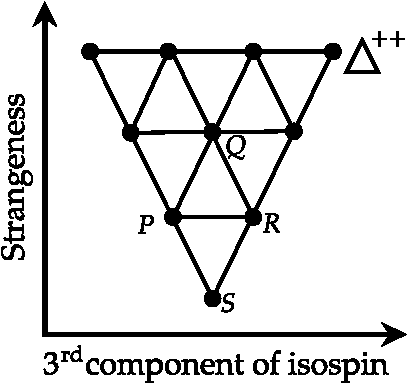
\includegraphics[height=4cm,width=4.5cm]{NP-13}
	\end{figure}
	\begin{tasks}(4)
		\task[\textbf{a.}]$P$
		\task[\textbf{b.}]$Q$
		\task[\textbf{c.}]$R$
		\task[\textbf{d.}] $S$ 
	\end{tasks}
	\begin{answer}$\left. \right. $
		\begin{figure}[H]
			\centering
			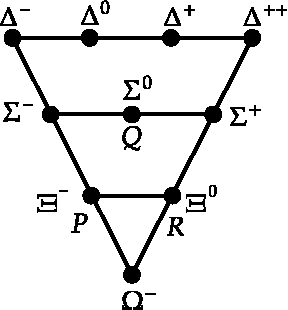
\includegraphics[height=4cm,width=3.8cm]{NP-17}
		\end{figure}
		So the correct answer is \textbf{Option (c)}
	\end{answer}
	\item  Considering baryon number and lepton number conservation laws, which of the following process is/are allowed?
	(i) $p \rightarrow \pi^0+e^{+}+v_e$\hspace{2cm}
	(ii) $e^{+}+v_e \rightarrow \mu^{+}+v_\mu$
	{\exyear{ 	GATE-2019}}
	\begin{tasks}(2)
		\task[\textbf{a.}]Both (i) and (ii)
		\task[\textbf{b.}]Only (i)
		\task[\textbf{c.}]Only (ii)
		\task[\textbf{d.}]Neither (i) nor (ii)
	\end{tasks}
	\begin{answer}
		\begin{align*}
		&\text{(i) }\quad p \rightarrow \pi^0+e^{+}+v_e\\
		&B: \quad+1 \quad 0 \quad 0 \quad 0:\text{ Not conserved}\\ 
		&\text{Therefore, this is not an allowed process}\\
		&\text{(II)}\quad e^{+}+v_e \quad \rightarrow \quad \mu^{+}+v_\mu\\
		&\begin{array}{lclcc}
		q: & +1 & 0 & +1 & 0: \text { conserved } \\
		\text { spin: } & 1 / 2 & 1 / 2 & 1 / 2 & 1 / 2: \text { conserved } \\
		L_e: & -1 & +1 & 0 & 0: \text { conserved } \\
		L_\mu: & 0 & 0 & -1 & +1: \text { conserved }
		\end{array}\\
		&\text{Since neutrino is involved, therefore parity is violated. This is allowed through weak interaction.}
		\end{align*}
		So the correct answer is \textbf{Option (c)}
	\end{answer}
	\item  A massive particle $X$ in free space decays spontaneously into two photons. Which of the following statements is true for $X$ ?
	{\exyear{ 	GATE-2019}}
	\begin{tasks}(1)
		\task[\textbf{a.}] $X$ is charged
		\task[\textbf{b.}]Spin of $X$ must be greater than or equal to 2
		\task[\textbf{c.}]$X$ is a boson
		\task[\textbf{d.}]$X$ must be a baryon 
	\end{tasks}
	\begin{answer}
		\begin{align*}
		&X \rightarrow \gamma+\gamma\\
		&q: \quad 0 \quad 0 \quad 0\\
		&\text{	spin: }0,1,2 \quad 1 \quad 1\\
		&\text{Thus spin of $X$ can be either 0,1 or 2 (integer).}\\
		&\text{Therefore, option (b) is wrong while option (c) is correct.}
		\end{align*}
		So the correct answer is \textbf{Option (c)}
	\end{answer}
	\item  Low energy collision ( $s$-wave scattering) of pion $\left(\pi^{+}\right)$with deuteron $(d)$ results in the production of two proton $\left(\pi^{+}+d \rightarrow p+p\right)$. The relative orbital angular momentum (in units of $\hbar$ ) of the resulting two-proton system for this reaction is
	{\exyear{ GATE-2019}}
	\begin{tasks}(4)
		\task[\textbf{a.}]0
		\task[\textbf{b.}]1
		\task[\textbf{c.}]2
		\task[\textbf{d.}] 3
	\end{tasks}
	\begin{answer}
		\begin{align*}
		&\pi^{+}+d \quad \rightarrow \quad p+p\\
		\text{Parity: }&(-1) \times(+1) \quad(-1)^l \quad \pi_p \pi_p\\ &\therefore\quad (-1)^l \pi_p \pi_p=-1\\
		&\text{Since }\pi_p=+1\\
		&\therefore\quad (-1)^l=-1\\
		&\text{Thus, }l=1.
		\end{align*}
		So the correct answer is \textbf{Option (b)}
	\end{answer}
	\item  A particle $Y$ undergoes strong decay $Y \rightarrow \pi^{-}+\pi^{-}$. The isospin of $Y$ is---------
	{\exyear{ GATE- 2020}}
	\begin{answer}
		\begin{align*}
		&\quad \quad  Y \rightarrow \pi^{-}+\pi^{-}\\
		&I: \quad 2 \qquad 1 \qquad 1\\
		&\text { In strong interaction, isospin is conserved, thus the isospin of } Y \text { is } 2 .
		\end{align*}
		So the correct answer is \textbf{2}
	\end{answer}
	\item  A particle $X$ is produced in the process $\pi^{+}+p \rightarrow K^{+}+X$ via the strong interaction. If the quark content of the $K^{+}$is $u \bar{s}$, the quark content of $X$ is
	{\exyear{	GATE- 2020}}
	\begin{tasks}(4)
		\task[\textbf{a.}]$c \bar{s}$
		\task[\textbf{b.}]und
		\task[\textbf{c.}]uus
		\task[\textbf{d.}]$u \bar{d}$ 
	\end{tasks}
	\begin{answer}
		\begin{align*}
		&\text{Lets first identify the particle $X$}\\
		&\pi^{+}+p \rightarrow K^{+}+X\\
		&\begin{array}{lllll}
		q:& +1&+1&+1&+1\\
		\text { spin: } & 0 & 1 / 2 & 0 & 1 / 2\\
		B:&  0&+1&  0&+1\\
		I: &0 &1 / 2& 1 & 1 / 2\\
		I_3: &+1&+\frac{1}{2}&+\frac{1}{2}&+1\\
		S:&  0 & 0 &+1&-1
		\end{array}\\
		&\text { Thus the particle } X \text { is } \Sigma^{+} \text {. The quark content of } \Sigma^{+} \text {is uus. Thus the correct option (c) }
		\end{align*}
		So the correct answer is \textbf{Option (c)}
	\end{answer}
\end{enumerate}
\colorlet{ocre1}{ocre!70!}
\colorlet{ocrel}{ocre!30!}
\setlength\arrayrulewidth{1pt}
\begin{table}[H]
	\centering
	\arrayrulecolor{ocre}
	\begin{tabular}{|p{1.5cm}|p{1.5cm}||p{1.5cm}|p{1.5cm}|}
		\hline
		\multicolumn{4}{|c|}{\textbf{Answer key}}\\\hline\hline
		\rowcolor{ocrel}Q.No.&Answer&Q.No.&Answer\\\hline
		1&\textbf{a} &2&\textbf{d}\\\hline 
		3&\textbf{b} &4&\textbf{d} \\\hline
		5&\textbf{b} &6&\textbf{d} \\\hline
		7&\textbf{a}&8&\textbf{a}\\\hline
		9&\textbf{c}&10&\textbf{c}\\\hline
		11&\textbf{d} &12&\textbf{d}\\\hline
		13&\textbf{b}&14&\textbf{d}\\\hline
		15&\textbf{c}&16&\textbf{c} \\\hline
		17&\textbf{c}&18&\textbf{b}\\\hline
		19&\textbf{2}&20&\textbf{c}\\\hline
	\end{tabular}
\end{table}